\chapter{Etude terrain} % 30 pages

	\paragraph{Comment j'ai réalisé mon étude terrain ? \\}

		Lors de mon étude terrain, j'ai eu l'occasion de recenser l'avis de nombreuses personnes sur l'open source mais également sur les réflexions menées lors de mon état de l'art.
		J'ai choisi d'orienter mes questions autour des 4 grands domaines qui représentent selon moi les piliers à batir pour valoriser l'open source, et sur lesquels l'éditeur a la main.

		\subparagraph{Etude quantitative \\}

		Pour cette étude terrain j'ai pu réaliser un sondage de 13 questions autour de ma problématique qui a pu être traitée par 40 personnes qui sont liées de près ou de loin à l'open source. Cette étude quantitative me permet de vérifier la véracité de mes hypothèses en cherchant le maximum d'approbations mais aussi de désapprobations de mes idées et réflexions.

		\subparagraph{Etude qualitative \\}

		L'étude qualitative que j'ai pu réalisé au travers de 4 interviews, m'a permise de confronter mes idées à celles d'autres personnes sensibles au domaine de l'open source . Ceci m'aide à étayer mes réflexions à travers leurs visions.

	\section{Plateforme d'hébergement}

		\subsection{Une interface pour communiquer qui laisse à désirer}

			Afin d'apporter plus de réflexions autour de mon hypothèse concernant l'amélioration de l'utilisation des plateformes pour les contributeurs, j'ai posé la question aux différentes personnes interrogées si le coté pratique de l'interface de ces plateformes leur convenait.\\

			Autour des plateformes qui contiennent et promouvoient l'open source, sur 39 réponses enregistrées pour cette question, 20 indiquent qu'il y a un manque à palier dans l'interface qui permet de communiquer avec l'éditeur open source. 

			\begin{figure}[!htb]
				\center
				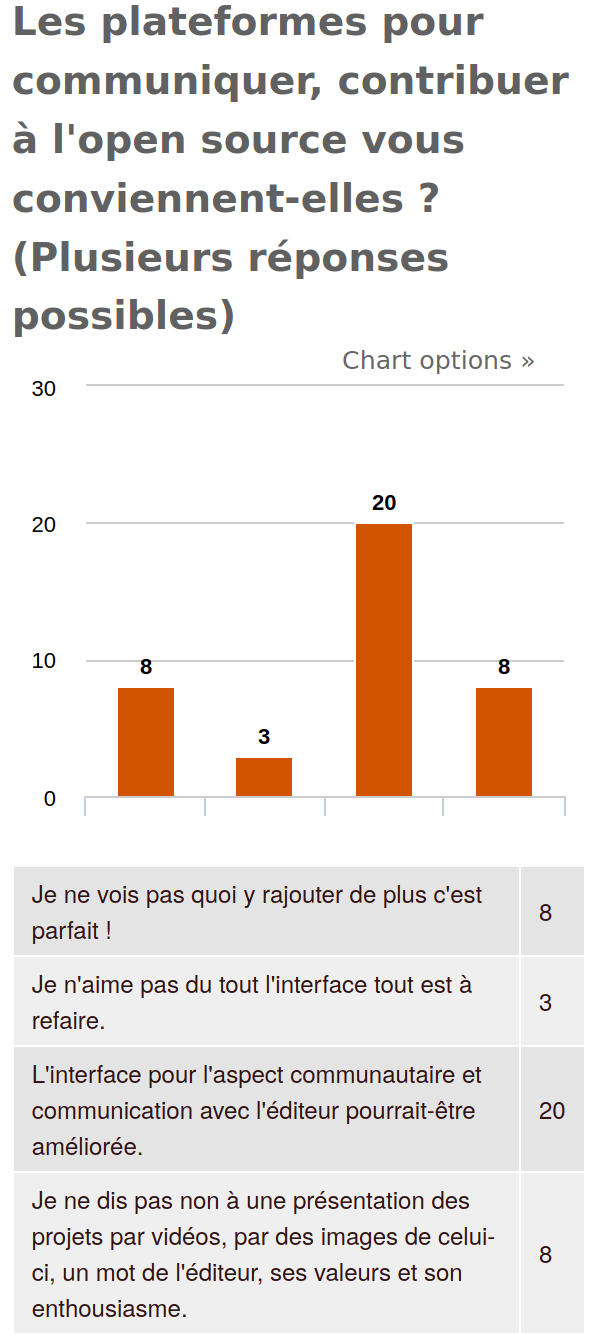
\includegraphics[scale=0.28]{./img/communicationediteur}
				\caption{Communication avec l'éditeur}
			\end{figure}

			Il apparait donc que \textbf{la communication qui a un aspect fondamental} pour l'open source \textbf{peut clairement être améliorée} afin de satisfaire non seulement les besoins dans la communication auprès de l'éditeur mais surtout le besoin du consommateur à communiquer correctement.\\

			Lors de l'interview auprès de Olivier \bsc{Mignial}, ingénieur systèmes embarqués chez l'une des plus grande entreprise promotrice de l'open source : SMILE. Celui-ci a déclaré : 

			\begin{center}
				\textit{
				\textquote{
					Pour \gls{mainliner} du code source, un processus décrit la manière de contribuer, et c'est le plus souvent par mail.(...) Linux, par exemple c'est entièrement du mail, on a des mailing lists extrêmement longues et des processus assez carrés !
				}
				}
			\end{center}

			Ce qui m'indique que \textbf{le système de gestion des contributions généralement présent est assez lourd}.\\

			Florent Garin, CEO de Docdoku et éditeur du logiciel open source DocdokuPLM, s'exprime sur le sujet en rapportant qu'il y a un problème sur ces plateformes pour communiquer avec les contributeurs:

			\begin{center}
				\textit{
				\textquote{
					On passe beaucoup de temps à éduquer les potentiels contributeurs car ils confondent contribution en relevant des anomalies et demandes de support (...) Un système de tag plus explicites sur les \gls{issues} améliorerait cette communication.
				}
				}
			\end{center}

			Finalement pour Florent Garin, un axe d'amélioration de l'éditeur auprès du contributeur serait la mise en place de guides, de documentations sur comment contribuer et d'un ticket spécial "first contribution".\\

			Ainsi, \textbf{des moyens peuvent être mis en oeuvre pour améliorer la communication sur les plateformes d'hébergement}.\\

			De plus la prise en main d'un logiciel open source est souvent compliquée nous révèle Quentin \bsc{Cazelle}, ingénieur logiciel chez Docdoku.\\

			Pourquoi selon lui ?

			\begin{center}
				\textit{
				\textquote{
					Car il y a des fonctionnalités non documentées (...) les plateformes sont incomplètes car les développeurs qui contribuent aux projets open sources ne s'embêtent pas à la documentation et a bien expliquer les issues.
				}
				}
			\end{center}

			J'en déduis donc qu'en plus d'une communication pouvant être améliorée, \textbf{faciliter l'écrit autour des contributions et sensibiliser les consommateurs à la documentation} est un axe d'amélioration potentiel.

		\subsection{Un module de présentation}

			Pour améliorer l'envie de contribuer à l'open source, je m'interroge sur le style de présentation des projets open source.\\
			Autour de la question sur le mode de présentation de l'open source, je souhaite m'informer sur la pertinence d'une présentation par vidéo du projet et de l'éditeur qui pourrait présenter son produit.\\
			Seulement 8 personnes sont intéressées pour avoir un présentation de ce type là.\\

			Lors de l'interview de Quentin \bsc{Cazelle}, Ingénieur développeur chez Docdoku, celui-ci mentionne tout de même le fait qu'une vitrine à ces plateformes s'impose pour les consommateurs finaux qui ne sont pas développeurs.

			\begin{center}
				\textit{
				\textquote{
					La plateforme est un frein pour l'utilisateur final non développeur, il faudrait en effet mettre une vitrine dans un style plus commercial (...)
				}
				}
			\end{center}

			En effet, pour les consommateurs finaux de logiciels open sources, les plateformes de développement et de contributions tel que Github ne sont pas familières et représentent un blocage pour l'utilisation.\\

			Florent \bsc{Garin}, mentionne quant à lui que le support de présentation par vidéo ne se prête pas à ce sujet.

			\begin{center}
				\textit{
				\textquote{
					La vidéo c'est souvent pour présenter des produits grands public, je pense pas que ce soit un bon moyen de communiquer sur l'open source car l'open source c'est majoritairement des projets ou des "briques" logicielles techniques.
				}
				}
			\end{center}

			J'en conclus qu'\textbf{une présentation du logiciel n'est pas forcément pertinente} pour le développeur contributeur ou les entreprises consommatrices.

		\subsection{Pas d'extrème sur les plateformes}

			Très peu de contributeurs, c'est-à-dire 8 sur 30, répondent que les plateformes sont parfaites et qu'ils ne voient pas d'amélioration potentielle.\\

			Il n'y a pas non plus beaucoup d'insatisfaits sur celles-ci car seulement 3 ont répondu que toute l'interface était à refaire.\\

			Je trouve donc que \textbf{les plateformes promotrices sont utilisées et essentielles} à l'open source et l'éditeur ne dois pas en faire l'impasse.

		\paragraph{Ce que j'en retire:\\}

		Les plateformes disponibles sur le marché sont utilisées par bon nombre d'entreprises et développeurs contributeurs à l'open source. Aucun besoin n'est ressenti compte tenu de l'aspect pratique de l'interface ou présentation des produits mais les modules pour échanger avec l'éditeur, le contributeur, le consommateur est un point négatif à l'open source.

	\section{Gestion des ressources}

		\subsection{Un mot de l'éditeur pour valoriser la contribution}

			Dans le but de faciliter l'envie des personnes potentiellement contributrices, j'ai posé une question concernant l'éditeur. "Est-ce qu'un espace de présentation de l'éditeur et de ses idéaux, valeurs et principes autour de ce produit open source serait une source de motivation à contribuer ?"\\

			Florent \bsc{Garin} mentionne qu'un projet open source est décentralisé et que malgré le leader potentiel (l'éditeur) qui approuve les contributions, l'open source n'est pas hierarchisé et donc ne se résume pas aux valeurs et missions de l'éditeur.

			\begin{center}
				\textit{
				\textquote{
					 (...), il y a un leader qui possède le répertoire avec le code mais ce n'est pas si hiérarchisé que cela, l'open source doit être vu comme un pot commun dans lequel tout le monde pioche.
					 Même si l'éditeur ou l'entreprise peut avoir un avantage financier, le projet est assez décorrélé d'elle, le code que je mets m'appartient quasiemment autant qu'à l'entreprise derrière (en fonction des licences), chacun doit chercher à contribuer dans le pot commun car ils se servent du logiciel et non car il incarne des valeurs.
				}
				}
			\end{center}

			Lors de l'interview de Quentin \bsc{Cazelle}, il souligne cette séparation de l'éditeur et de la communauté.
			\begin{center}
				\textit{
				\textquote{
					 Ce n'est pas une entreprise qui a un besoin, c'est une communauté avec des besoins !
				}
				}
			\end{center}

			Il n'y a donc finalement pas vraiment d'échanges avec les valeurs et missions de l'initiateur du projet open source \textbf{mais une communication autour du besoin du consommateur sur ce projet open source}

		\subsection{Pas de niveau hiérarchique}

			Concernant la gestion des ressources et notemment la gestion humaine dans les projets open sources, je m'interroge sur la relation entre l'éditeur et sa communauté. Et sa manière de gérer les contributeurs potentiels.

			Lors de mon interview avec Quentin \bsc{Cazelle}, il m'informe que les relations hiérarchiques dans l'open source sont plutôt implicites.

			\begin{center}
				\textit{
				\textquote{
	 				Si j'arrive sur un projet open source et que les gens connaissent bien le projet, il sont "au dessus" de moi, si moi, je monte en compétence alors ma voix vaudra la leur. (...) Ce sont des rapports qui se construisent implicitement, cela se joue au mérite. (...) L'éditeur au final c'est juste lui qui a le dernier mot pour intégrer la contribution.
				}
				}
			\end{center}

			Ce qui rejoint le point de vue de Florent \bsc{Garin}, qui m'informe que la relation hiérarchique dans un projet open source est inexistante, l'éditeur ne peux pas contrôler les contributeurs, ni assigner de tâches (ce que je précise ultérieurement).\\

			J'en conclus \textbf{qu'il n'y a pas de hiérarchie autour de l'open source mais seulement des échanges} entre la communauté et l'éditeur.

		\subsection{La gestion des projets open sources}

			Autour de ma deuxième hypothèse sur l'optimisation des ressources (principalement humaines), je sollicite l'avis des personnes concernant leur éventuelle participation à l'open source.\\

			J'ai donc demandé aux personnes interrogés de s'imaginer, en tant qu'éditeur open source, le meilleure modèle de développement de projet.\\

			Ainsi en tant qu'éditeur, qu'aimeraient-ils de leur communauté concernant leur participation ?\\

			28 personnes sur 39 ont ainsi répondu qu'ils aimeraient se mettre au même niveau que la communauté et qu'en tant qu'éditeur ils contribuent de la même façon que la communauté.\\

			Seulement 10 ont répondu qu'ils aimeraient se charger du noyau et que le développement de modules et d'extensions à intégrer est attribué à la communauté.\\

			1 seule personne à répondu qu'elle n'aimait pas l'aspect communautaire de l'open source.

			\begin{figure}[!htb]
				\center
				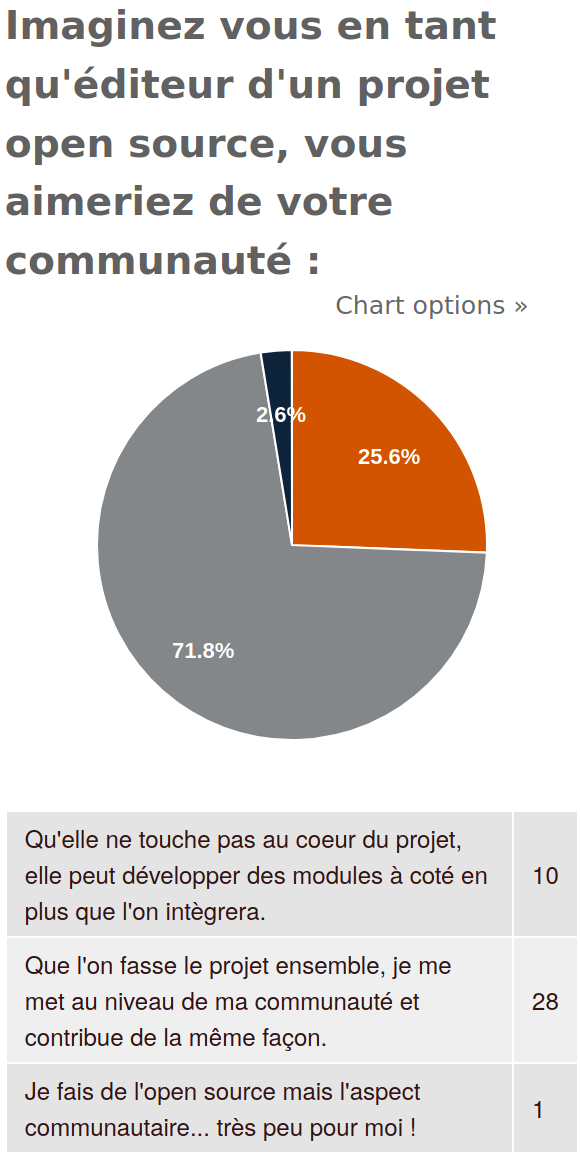
\includegraphics[scale=0.28]{./img/gestioncommunaute}
				\caption{Gestion de communauté en tant qu'éditeur}
			\end{figure}

			\newpage

			Quentin \bsc{Cazelle} lui, exprime que les besoins dans le modèle de noyau/extension sont tous différents pour chaque contributeur ou consommateur et cela pose un problème de simplicité du logiciel qu'il est difficile de gérer.

			\begin{center}
				\textit{
				\textquote{
					 Il peux y avoir des besoins contradictoires, qui ramènent beaucoup de complexité, dans mon ancienne société, notre besoin était simple et le logiciel est devenus 4 fois trop gros, il est difficile de séparer le noyau des extensions car l'intégrité du code n'est pas garantie, les mises à jours peuvent être compliqués.
				}
				}
			\end{center}

			De plus il souligne que les extensions pour des besoins spécifiques deviennent intéressant à vendre alors qu'une modification du coeur du projet doit être partagée à l'ensemble de la communauté.\\

			J'en déduis qu'un mode de gestion noyau/extension n'est pas forcément bien perçu ou logique pour les personnes interrogés et que l'aspect de communauté et de management horizontal est mieux à leurs yeux. Ainsi \textbf{travailler de pair avec l'éditeur sans impression de dénivelé de pouvoir est préférable}.\\

			Florent \bsc{Garin} mentionne quant à lui qu'il y a plusieurs business models autour de l'open source mais qu'ils ont très peu de succès.

			\begin{center}
				\textit{
				\textquote{
					 Dans les business models présents, il y a celui ou les développeurs se réunissent autour d'un besoin commun et réalisent un projet open source à but non lucratif et c'est souvent ce qui marche le mieux finalement. Comme pour le noyau linux, personne ne gagne de l'argent directement avec celui-ci, et c'est la mutualisation d'un effort commun qui prime.
				}
				}
			\end{center}

			Egalement, selon lui, ce modèle noyau/extension ne prévaut pas, il faut faire attention aux entreprises "prédatrices" qui mettent à mal ces projets.

			\begin{center}
				\textit{
				\textquote{
					 Des exemples, il y en a plein, je pense à Docker qui a crée son projet open source, a essayé de développer ses extensions et qui finalement n'a pas vraiment réussi à monétiser cela face à d'autres entreprises avec d'autre aspirations comme Google qui a bien profité de Docker. (...)
				}
				}
			\end{center}

			Aucun modèle n'est mieux qu'un autre souligne Quentin \bsc{Cazelle}, les besoins de l'éditeur varient et il jongle parfois entre autoriser les contributions au coeur de son projet ou accepter les extensions proposées.\\

			Ainsi, je peux en déduire qu'il y a beaucoup de menaces et contraintes autour des projets open sources et \textbf{les business models à employer ne se résument pas à un seul type qui fonctionnera généralement}.

		\subsection{La gestion des contributions}

			Afin de gérer les ressources mise à disposition et donc essentiellement la communauté, j'ai posé la question sur comment en tant que membre d'une communauté open source, la personne aimerait travailler.\\

			A celle-ci, 80\% des personnes ont répondues qu'elles préfèrent toucher un peu à tout dans le projet et gagner en connaissance en sollicitant une multitude de personnes.\\

			Seulement 20\% des personnes souhaiteraient monter en compétence dans un seul domaine et y être attribué pour plus de ciblage sur une compétence clé.

			\begin{figure}[!htb]
				\center
				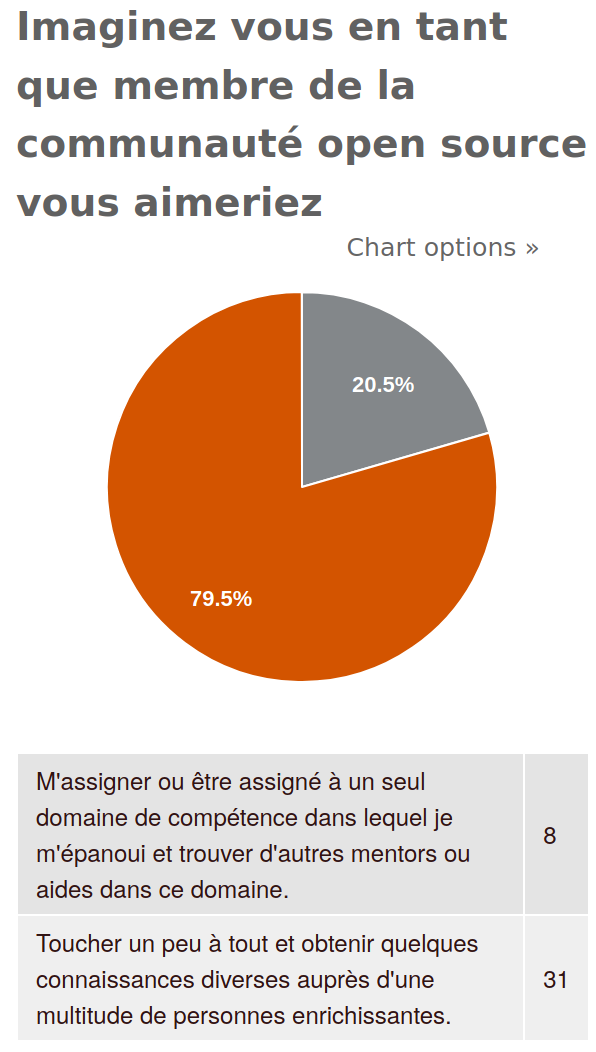
\includegraphics[scale=0.28]{./img/multicompetence}
				\caption{Multi-compétence ou expertise ?}
			\end{figure}

			Pour Quentin \bsc{Cazelle}, le fait de toucher à tout lui est préférable pour une raison principale:

			\begin{center}
				\textit{
				\textquote{
					 Cela donne une meilleure compréhension globale du produit, sur le projet open source auquel j'ai participé, j'ai touché à tout et cela m'a permis de pouvoir expliquer le fonctionnement de tout le logiciel en entier.
				}
				}
			\end{center}

			La vision du contributeur est donc de gagner un peu en compétence dans tout les domaines afin d'être polyvalent plutôt qu'expert dans un domaine précis.\\

			Florent \bsc{Garin} souligne un fait important lors de cette question autour de la gestion des ressources.\\

			L'open source c'est selon le bon vouloir du contributeur, il n'y a pas de relation hiérarchique, ni de tâche à donner aux contributeurs de ce fait on ne peux pas assigner les contributeurs à un domaine spécifique plutôt qu'à un autre. Ainsi tout dépend de la volonté du contributeur.

			\begin{center}
				\textit{
				\textquote{
					 Chacun est libre de faire ce qu'il veut, par contre en tant qu'éditeur, tu es libre d'accepter sa contribution,(...) néanmoins celui qui va contribuer sur un domaine qu'il ne maitrise pas se verra peut être refuser plusieurs fois des contributions.
				}
				}
			\end{center}

			Ainsi \textbf{cela change ma vision sur l'optimisation des ressources humaines et des contributions que je perçevais comme "assignable"} mais qui restent au bon vouloir du contributeur.

		\paragraph{Ce que j'en retire:\\}

			Même si l'on prône l'aspect communautaire de l'open source, il ne s'agit pas d'une micro entreprise avec un leader dirigeant, tout est basé sur la volonté du contributeur.\\ Également, le business model de réalisation d'un produit open source est à adapter selon le produit, les contributeurs et tout les éléments dans cet écosysteme.

	\section{Chez le consommateur}

		\subsection{La contribution du consommateur}

			Afin de mieux orienter mon hypothèse concernant les besoins et envies des consommateurs qui planent sur l'open source et manquent d'être mieux exprimés, je me pose la question sur l'intérêt qu'ont les individus interrogés autour de l'open source.\\

			Je leur ai donc demandé: "Avez-vous déjà contribué à l'open source ?"

			Dans les personnes interrogés, 60\% y ont déjà contribué, 28\% souhaitent y contribuer un jour.

			\begin{figure}[!htb]
				\center
				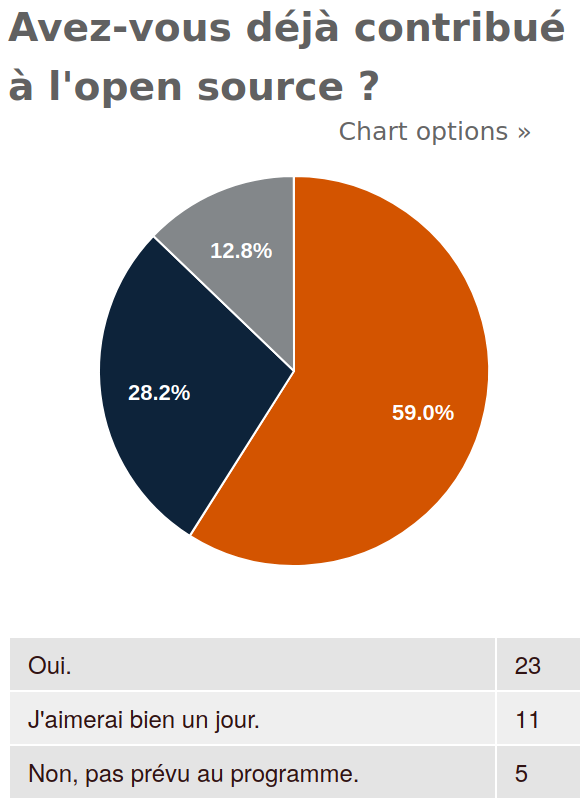
\includegraphics[scale=0.28]{./img/contribution}
				\caption{Contribution à l'open source}
			\end{figure}

			L'open source est donc un sujet qui les intéresses et dont \textbf{ils peuvent ou veulent investir du temps en y contribuant}.\\

			\newpage
			Et ce quelque soit le domaine d'activité de leur entreprise. Pour cibler un peu mieux les personnes questionnées, j'ai souhaité savoir quel était le domaine d'activité principal de leurs entreprise.\\

			Sur les 37 personnes qui ont répondues, je note une diversité des domaines d'activités:

			\begin{itemize}[label=\textbullet, font=\LARGE \color{burntorange}]
				\item Edition, Communication, Multimédia
				\item Etude et conseils
				\item Informatique / Télécom
				\item Industriel
				\item Autres
			\end{itemize}

			\begin{figure}[!htb]
				\center
				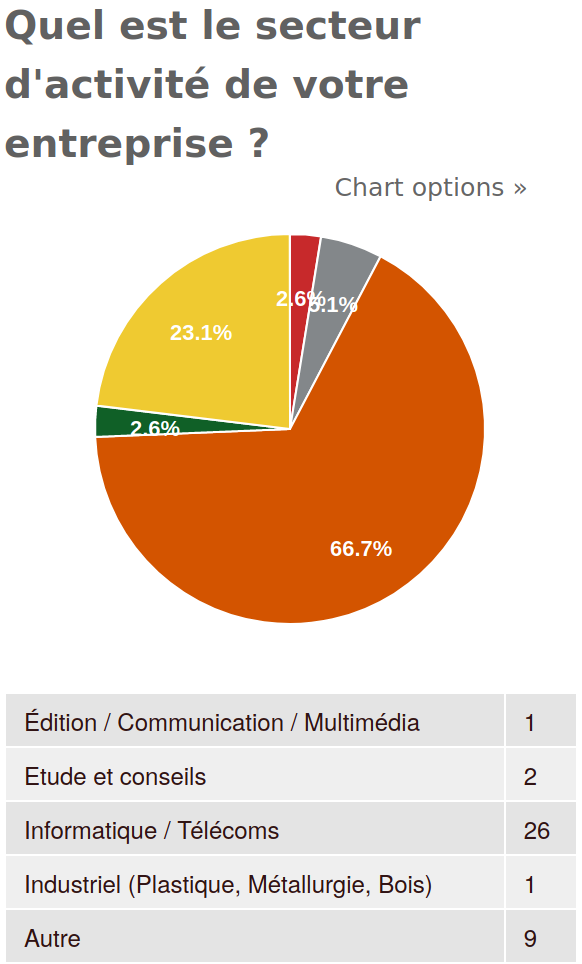
\includegraphics[scale=0.28]{./img/secteuractivite}
				\caption{Secteur d'activité des personnes interrogées}
			\end{figure}

			\newpage

			Ainsi \textbf{l'open source n'est pas seulement présent dans les entreprises informatiques} et est une préoccupation pour les personnes interrogés.\\

			Et c'est ce que souligne Olivier \bsc{Mignial}, dans notre interview qui précise la place importante de l'open source.

			\begin{center}
				\textit{
				\textquote{
		 			Dans le monde de l'entreprise on entend énormément parler de l'open source, c'est d'autant plus important pour les petites entreprise comme les startups que pour les grosses car on ne peut pas perdre de temps à réinventer la roue.
				}
				}
			\end{center}

		\subsection{Le ressenti du consommateur à contribuer}

			En relation avec mon hypothèse sur l'envie et le besoin de contribuer, j'ai posé une question dans mon questionnaire autour de la perçeption que les gens peuvent avoir dans l'accueil de contributions: ont ils des peurs qui les freinent ou au contraire est-ce agréable de partager leur travail et d'aider l'editeur et la communauté.\\

			Globalement, aucun frein n'est ressenti à la contribution et son accueil par l'éditeur, même si ces personnes ne contribuent par pour autant:

			\begin{itemize}[label=\textbullet, font=\LARGE \color{burntorange}]
				\item 46\% des interrogés ont répondu que leurs contributions étaient très bien accueillies, que l'éditeur et la communauté étaient agréable.
				\item 43\% Ne prennent pas le temps de contribuer mais n'y voient aucun blocage.
				\item Et seulement 11\% ont peur de contribuer et d'être jugé.
			\end{itemize}

			\begin{figure}[!htb]
				\center
				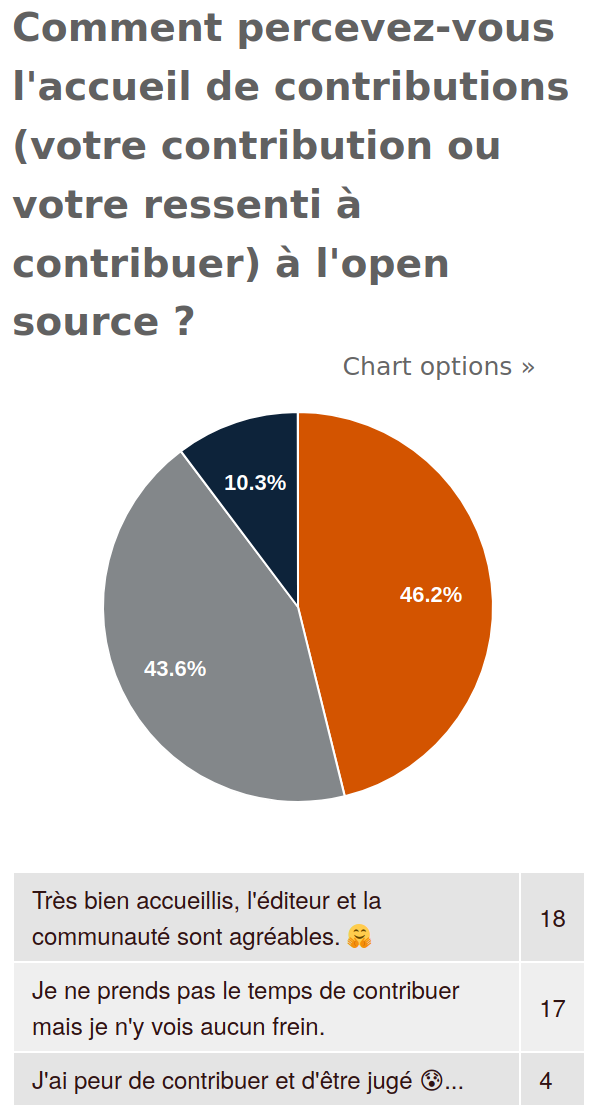
\includegraphics[scale=0.28]{./img/perception}
				\caption{Perception de contributions à l'open source}					
			\end{figure}

			J'en déduis que la moitiée des personnes ont besoin de \textbf{plus de motivations et de nécessités à contribuer}.\\

			Dans leur entreprise, ces personnes considèrent pourtant majoritairement que l'open source est essentiel ou nécessaire.\\

			Pour 10 personnes, l'open source est essentiel et ils y attachent beaucoup d'importance.
			13 questionnés disent que l'open source est nécessaire dans leur projets. 8 personnes disent que leur entreprise ne s'en soucie pas vraiment et 5 personnes n'ont jamais entendu parlé d'open source dans leur société.\\


			Je m'aperçoit que \textbf{malgré le degré d'importance considéré de l'open source les personnes interrogés n'en font pas une affaire personnelle}.

			\begin{figure}[!htb]
				\center
				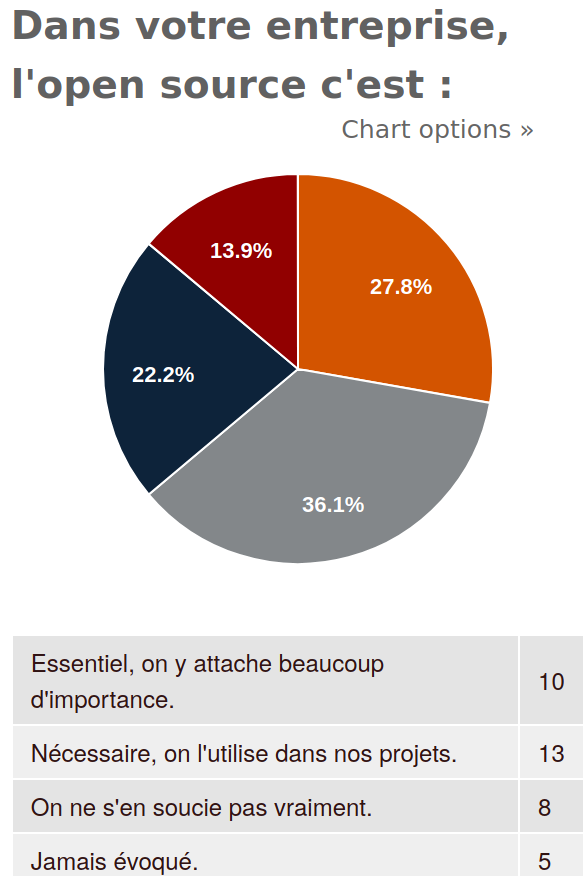
\includegraphics[scale=0.28]{./img/importanceos}
				\caption{L'importance de l'open source}					
			\end{figure}


			Florent \bsc{Garin} souligne que les personnes charitables qui souhaitent contribuer ne doivent pas tant être sensibilisés mais guidés sur la manière de contribuer.\\

			Lors de cette interview , il m'informe également, du manque de contribution général présent dans l'open source, et du manque de volonté à contribuer

			\begin{center}
				\textit{
				\textquote{
					On ne peux pas sensibiliser une entreprise à participer à un projet open source, l'entreprise va là ou le profit l'appelle.
				}
				}
			\end{center}

			Il explique donc un axe pour inciter les entreprises à contribuer à l'open source:

			\begin{center}
				\textit{
				\textquote{
		 			Il faut plutôt essayer de bâtir des règles où les entreprises sont incités à contribuer, non pas par acte de bienveillance, mais parce que financièrement et économiquement elles ont des motivations à contribuer.
				}
				}
			\end{center}

			Olivier \bsc{Mignial} rajoute à ce propos que c'est souvent difficile pour une entreprise de comprendre l'intérêt qu'elle a à ouvrir son code et de contribuer au monde de l'open source et pourtant il est réel.

			\begin{center}
				\textit{
				\textquote{
					Open sourcer son code c'est quand même un peu de temps, un peu d'énergie et il n'y a pas cette volonté la de la part des entreprises (...) néanmoins la contribution à l'open source peut jouer des enjeux économiques.Elle permet d'être connecté aux autres produits et logiciels et apporte également une meilleure visibilité de son produit sur le marché.
				}
				}
			\end{center}

			Florian \bsc{Gasc}, architecte logiciel chez Simplifia, déclare que l'open c'est avant tout une model économique.

			Il me confie:

						\begin{center}
				\textit{
				\textquote{
					Il faut avoir en tête que si l'entreprise est suffisamment grosse, l'open source lui fourni un pouvoir de control, une main mise sur une grosse parti du marché comme pour Chrome, Android, Kubernetes et bien d'autres(...) L'idée est simple: l'Open source est pratique, si tu arrives à l imposer au plus grand nombre, tu profites de la communauté pour générer de l'argent (ou en économiser).			
					}
				}
			\end{center}

			La contribution des entreprises à l'open source devient essentielle pour les enjeux futurs de l'IT. Ainsi il \textbf{reste encore du chemin pour amener les gens à participer et contribuer} activement à l'open source.

		\subsection{Un besoin écouté}

			J'ai abordé le sujet de l'écoute des besoins, des remarques faites par le consommateur qui remontent à l'éditeur afin de m'approcher de mon hypothèse sur les envies et besoins des consommateurs.\\

			30 des 39 personnes interrogées ont trouvés qu'après une demande auprès d'un éditeur open source, le besoin du consommateur est suffisemment écouté.

			\begin{figure}[!htb]
				\center
				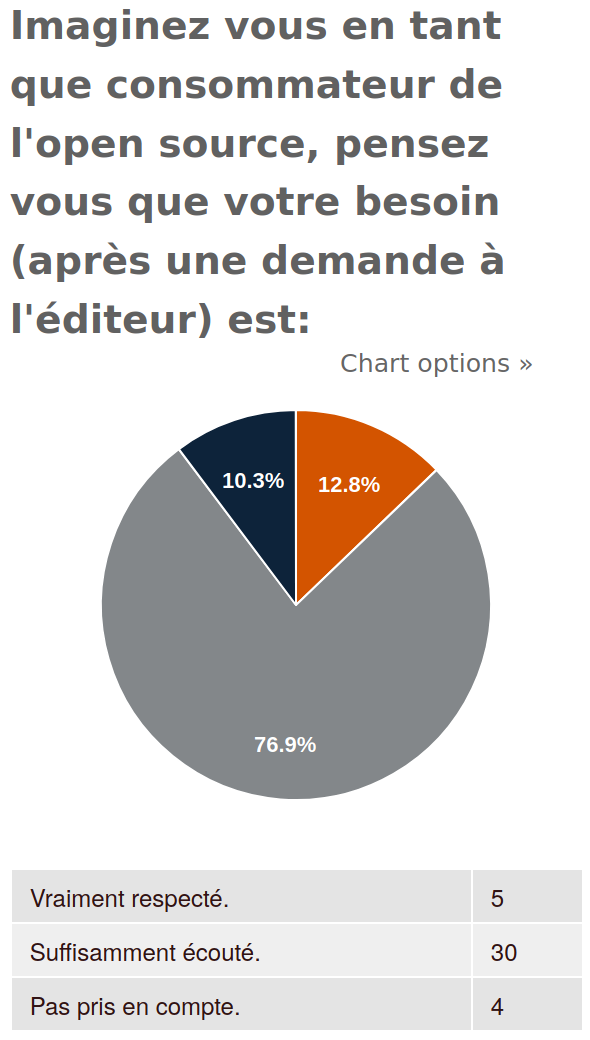
\includegraphics[scale=0.28]{./img/ecoutebesoin}
				\caption{Ecoute du besoin du consommateur}
			\end{figure}

			Ainsi \textbf{le manque de communication dans l'expression du besoin dans l'open source ne relève pas d'un problème de communication humaine mais d'outils techniques}.

			\newpage

			Selon Quentin \bsc{Cazelle}, l'accueil des demandes, remarques à l'éditeur est généralement bien perçu.

			\begin{center}
				\textit{
				\textquote{
		 			Sur les sites comme Stackoverflow, Github, du moment que les questions sont respectueuses et utiles, les réponses sont constructives et on est bien accueilli.
				}
				}
			\end{center}

			Pour Florent \bsc{Garin}, en tant qu'éditeur logiciel open source, le besoin du consommateur est entendu et si plusieurs personnes remontent ce besoin alors l'éditeur peut supposer qu'il y a un marché intéressant derrière.\\

			Il faut néanmoins garder à l'esprit, selon lui, qu'il n'y a pas de relations donnant-donnant.

			\begin{center}
				\textit{
				\textquote{
		 			Personne ne doit rien à personne dans cette histoire, les éditeurs ne doivent rien aux consommateurs et vice-versa.
				}
				}
			\end{center}

		\paragraph{Ce que j'en retire:\\}

		Le consommateur de l'open source est généralement bien au courant de l'intérêt et des enjeux inhérents à l'open source pour le monde de l'informatique, et malgré cela, il n'est pas lié à l'open source. Cela va du bon sens, de la générosité de sa part à contribuer ou de son intérêt économique.\\

		Le consommateur \emph{prends}, \emph{utilise}, mais ne contribue pas ou peu. Ainsi, il ne faut pas se tourner vers le consommateur pour qu'il \emph{rende} au monde ce qu'il a pris. Les entreprises ont encore du mal a voir les enjeux lié à l'open source et le besoin d'y donner un peu de leur travail pour que l'informatique en bénéficie.

	\section{Marketing de l'open source}

		\subsection{L'école et l'open source}

			\subsubsection{la présence de l'open source}

				Promouvoir l'open source fait partie intégrante de mes hypothèses.Qu'il s'agisse de l'entreprise, d'un éditeur ou de l'école, il me paraît essentiel de faire comprendre aux personnes liées à l'informatique de l'importance de l'open souce. \\
				J'ai donc posé une première question concernant la présence de l'open source dans les écoles informatiques.

				Sur une trentaine de personnes qui ont répondu à la question: "Devrait on sensibiliser les gens à l'open source dans les écoles informatiques ?", je constate que 13 de ces personnes ont découvert l'open source par le biais de l'école.

				\begin{figure}[!htb]
					\center
					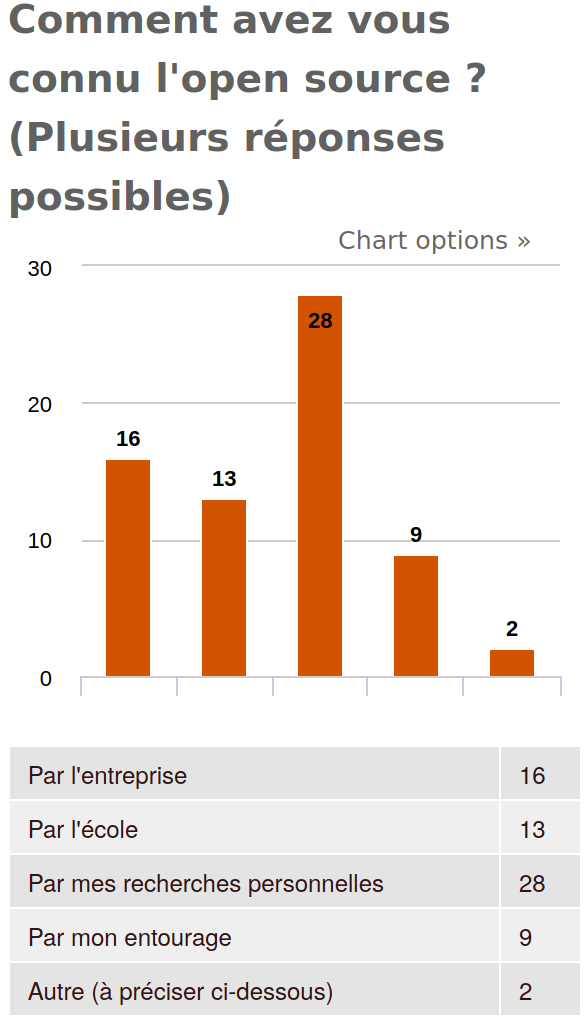
\includegraphics[scale=0.28]{./img/decouverte}
					\caption{Découverte de l'open source}
				\end{figure}

				A ceci, Quentin \bsc{Cazelle}, qui sort d'une école d'informatique m'indique que son école traitait bien de l'open source et que le sujet était bien présent:

				\begin{center}
					\textit{
					\textquote{
						A l'IUT, j'ai eu des cours sur l'open source, c'était suffisant pour comprendre le concept (...) c'est peut-être le minimum que l'on puisse traiter sur ce sujet mais c'est nécessaire. 
					}
					}
				\end{center}

				Rémi \bsc{Buhler}, développeur logiciel, était récemment dans une école informatique et selon lui le sujet n'a pas vraiment été traité.

				\begin{center}
					\textit{
					\textquote{
			 			J'ai entendu parlé de l'open source à l'école dans le cadre de la propriété intellectuelle, mais l'on ne m'a jamais vraiment appris tout ce qui se trouve derrière l'open source et son utilisation à travers le développement logiciel.
					}
					}
				\end{center}

				Également, plus de la moitié des personnes, soit 22 interrogées, ont répondues sur que l'open source était peu ou tout juste assez évoqué à l'école.\\

				9 personnes trouvent que les écoles informatiques traitent suffisamment de l'open souce\\

				Seulement 3 personnes ont déclaré que l'open source était fortement présent dans les écoles informatiques.

				\begin{figure}[!htb]
					\center
					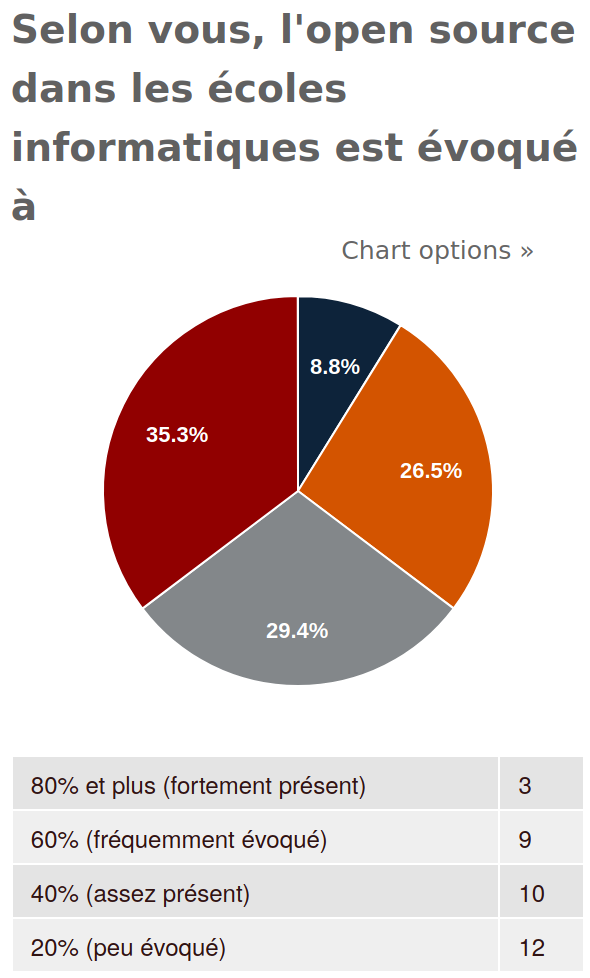
\includegraphics[scale=0.28]{./img/osalecole}
					\caption{L'open source à l'école}					
				\end{figure}

				Ce manque de présence de l'open source m'a également été rapporté par Olivier \bsc{Mignial} lors de notre rencontre:

				\begin{center}
					\textit{
					\textquote{
			 			L'aspect codeur du dimanche et instable de l'open source, c'est aussi une impression que j'avais à l'école car on en entend très peu parler.
					}
					}
				\end{center}

				Ainsi l'open source n'est pas vraiment présent dans les écoles informatiques et si il l'est, alors il n'est que vaguement évoqué.

			\subsubsection{Sensibiliser à l'open source}

				Après avoir questionné sur la présence de l'open source dans les écoles, j'ai poursuivi ma recherche d'informations sur cette sensibilisation à l'open source et la pertinence de celle-ci dans les écoles informatiques.

				Sur une trentaine de personnes qui ont répondues à la question: "Devrait on sensibiliser les gens à l'open source dans les écoles informatiques ?"\\

				Une majoritée des contributeurs, soit 92\% mentionne que l'on devrait bel et bien sensibiliser les gens à l'open source dans les écoles informatiques\\

				Seulement 3 personnes, dont 2 qui ont découverts l'open source à l'école, trouvent que c'est déjà fait intrinsèquement au programme.\\

				\begin{figure}[!htb]
					\center
					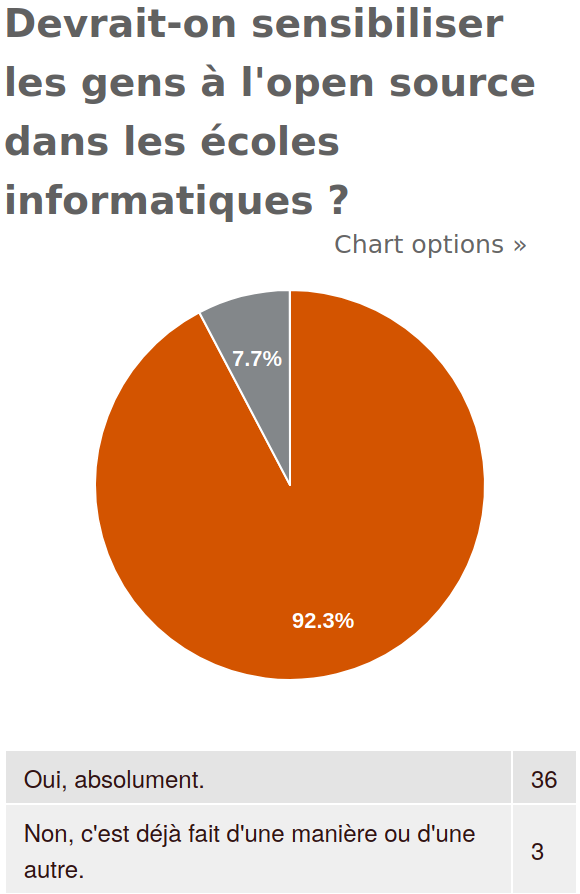
\includegraphics[scale=0.28]{./img/sensibiliser}
					\caption{Sensibiliser à l'open source}
				\end{figure}

				Quentin \bsc{Cazelle} me dit que l'open source est une brique nécessaire pour le métier de développeur logiciel et donc les étudiants en informatique.

				\begin{center}
					\textit{
					\textquote{
						Quelqu'un qui fait 5 années d'études de développeur et ne sait pas ce qu'est l'open source, c'est une abération!
					}
					}
				\end{center}

				Pour Florent \bsc{Garin}, il n'y a pas véléité à sensibiliser le monde à l'open source, mais ils doivent bien connaitre au passage, s'ils sont dans une école informatique, ce qu'est l'open source.\\

				C'est également l'avis d'Olivier \bsc{Mignial} qui rajoute:

				\begin{center}
					\textit{
					\textquote{
						L'open source on en entend très peu parler au niveau grand public pour autant est-ce qu'il y a une réelle importance à le faire (...)  Linux n'est pas promu au grand public et pourtant c'est l'OS le plus utilisé au monde en entreprise.
					}
					}
				\end{center}

				J'en conclus que \textbf{l'open source est intrinsèque au métier de développeur et de l'entreprise mais qu'il n'y a pas une grande importance à sensibiliser tout le monde à ce sujet} et qu'il est préférable donc de \textbf{cibler les futurs contributeurs} et employés de demain.\\

				\newpage

		\subsection{Le support payant}

			Afin de vérifier si la perception de gratuité que l'on a de l'open source et le fait de vendre du support, ne soit pas mal vu par le consommateur, je leur pose la question de la pertinence de ce support logiciel.\\

			Dans l'ensemble des personnes interrogés, une forte majorité indiquent qu'ils ne sont pas contre payer du support pour un logiciel open source. \\

			13 personnes ont répondues qu'il était nécessaire d'avoir du support et le prix est abordable en général. 23 personnes n'ont pas d'objection à payer pour du support logiciel et comprennent qu'il faille rémunérer l'éditeur d'une certaine façon. Et seulement 3 ont répondu qu'ils pensaient que l'open source devait être gratuit.

			\begin{figure}[!htb]
				\center
				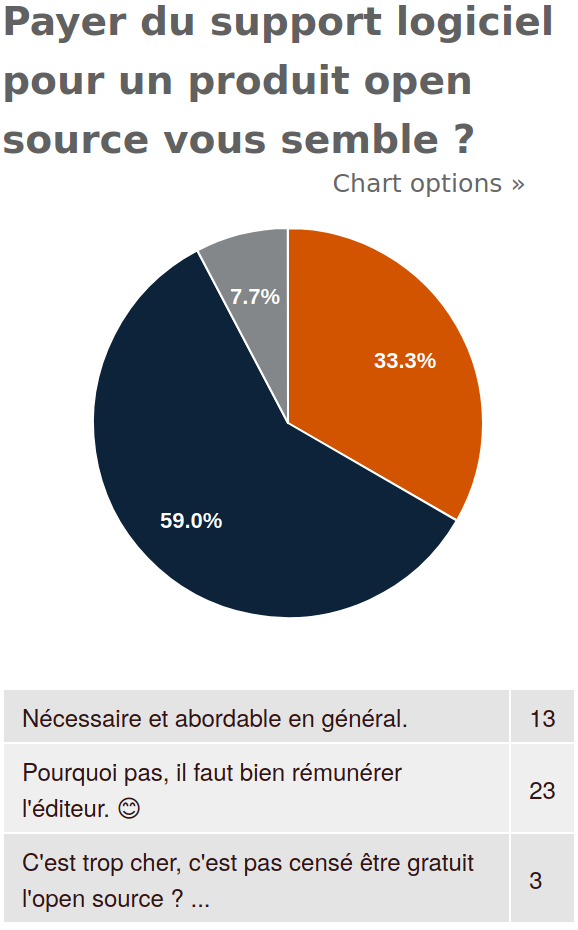
\includegraphics[scale=0.28]{./img/payersupport}
				\caption{Payer du support logiciel}					
			\end{figure}


			"L'open source attire beaucoup pour sa gratuité" déclare Florent \bsc{Garin} et il cible un problème important dans l'abus de ces consommateur qu'ils désigne par le terme de "\gls{leechers}"
			\begin{center}
					\textit{
					\textquote{
						Les consommateurs remontent des anomalies qui ne sont en réalité pas des anomalies mais des demandes de support
					}
					}
				\end{center}

			C'est donc que le modèle économique de l'éditeur à travers \textbf{la vente de support logiciel n'est pas un frein à la consommation de l'open source}.

		\subsection{Le marketing classique}

			Autour de la sensibilisation à l'open source j'ai posé la question aux personnes interviewées, si d'un point de vue marketing il est nécessaire de promouvoir son produit open source malgré la promotion inhérente à l'open source.

			Florent \bsc{Garin}, qui est éditeur d'un logiciel open source, mentionne à ce sujet:

			\begin{center}
					\textit{
					\textquote{
			 			Derrière le projet open source il y a finalement un marketing classique qu'il faut faire pour survivre, on espère que le projet open source va suffir de lui même mais ce n'est pas le cas.					
			 			}
					}
			\end{center}

		\subsection{Promouvoir son produit en l'open sourçant}

			Enfin pour améliorer cet aspect marketing et publicitaire de l'open source, lors de mon interview avec Olivier \bsc{Mignial}, nous échangeons autour des avantages qu'apporte l'open source.\\

			Il est, selon lui, de l'intérêt des éditeurs d'open sourcer leur code afin d'y rajouter une brique d'interopérabilités avec les autres produit ce qui permettra de mieux vendre ses produits.

			\begin{center}
				\textit{
				\textquote{
		 				Il peut être intéressant d'open sourcer des produits pour le coté interropérable(...), pour peu qu'un concurrent ait sorti quelque chose de meilleur, il vaut mieux que vos produits soient interropérables pour quand même vendre une partie de ceux-ci.
		 			}
					}
			\end{center}


			\paragraph{Ce que j'en retire:\\}

				L'open source possède de nombreux avantages en matière d'aspect économique pour les entreprises, tant par l'accessibilité à moindre coût pour les consommateurs, que pour le gain en interropérabilité, en interfaçage avec les différents produits du marché ou l'on peut s'y frayer un chemin. Mais pour tout ces bénéfices, on se doit de sensibiliser les entreprises, les développeurs afin de leur rappeler les enjeux de leurs contributions dans l'open source.









